\documentclass[border=6pt]{standalone}
\usepackage{tikz}
\usetikzlibrary{arrows.meta, calc}

\definecolor{hawk}{HTML}{D55E00}
\definecolor{dove}{HTML}{0072B2}
\definecolor{crit}{HTML}{555555}

\begin{document}
\pagecolor{white}
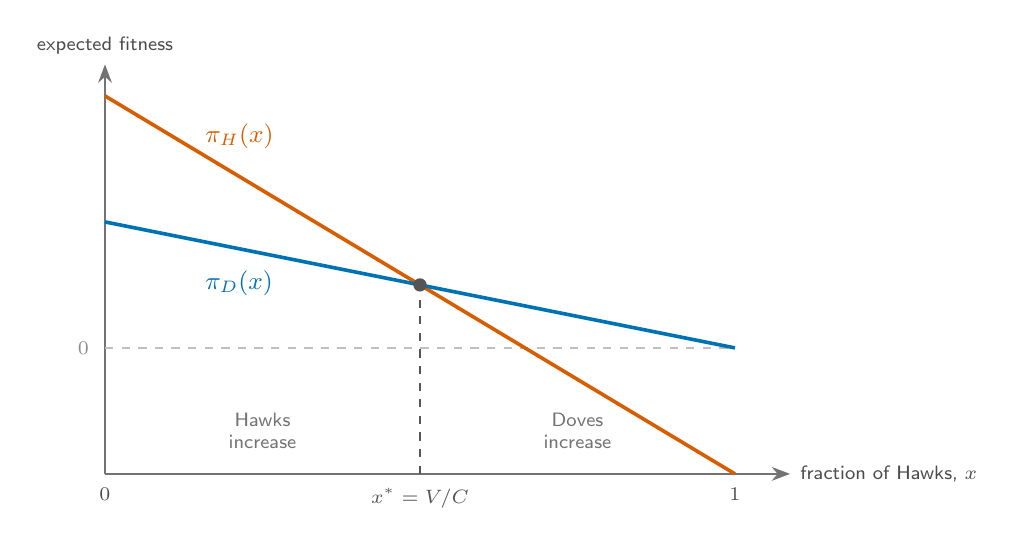
\begin{tikzpicture}[
    >=Stealth, font=\sffamily,
    lab/.style={font=\sffamily\scriptsize, text=black!70},
]
% data point (x,y) with x in [0,1], fitness y in [-1,2] maps to
%   (x*8, 1.6 + y*1.6)
\def\yz{1.6}
\def\ys{1.6}

% axes
\draw[->, line width=0.8pt, black!55] (0,0) -- (0,5.2)
    node[above, lab]{expected fitness};
\draw[->, line width=0.8pt, black!55] (0,0) -- (8.7,0)
    node[right, lab]{fraction of Hawks, $x$};

% fitness = 0 reference
\draw[black!25, dashed, line width=0.6pt] (0,\yz) -- (8,\yz);
\node[lab, anchor=east, text=black!45] at (-0.08,\yz) {$0$};

% Hawk line: (0,2) -> (1,-1)
\draw[hawk, line width=1.3pt] (0,{\yz+2*\ys}) -- (8,{\yz-1*\ys});
% Dove line: (0,1) -> (1,0)
\draw[dove, line width=1.3pt] (0,{\yz+1*\ys}) -- (8,{\yz+0*\ys});

% crossing at (0.5,0.5) -> (4, 2.4)
\draw[crit, dashed, line width=0.8pt] (4,0) -- (4,2.4);
\fill[crit] (4,2.4) circle (2.4pt);

% axis ticks / labels
\node[lab, anchor=north] at (0,-0.06) {$0$};
\node[lab, anchor=north] at (8,-0.06) {$1$};
\node[lab, anchor=north, text=crit] at (4,-0.06) {$x^{*}=V/C$};

% curve labels
\node[hawk, font=\sffamily\small, anchor=south west] at (1.15,4.0) {$\pi_H(x)$};
\node[dove, font=\sffamily\small, anchor=north west] at (1.15,2.7) {$\pi_D(x)$};

% region annotations
\node[lab, text=black!55, align=center] at (2,0.55) {Hawks\\ increase};
\node[lab, text=black!55, align=center] at (6,0.55) {Doves\\ increase};

\end{tikzpicture}
\end{document}
